\xchapter{Planejamento do estudo experimental}
{...}
\label{planejamento}

Os estudos apresentados no Capítulo \ref{fundamentacao} mostram carência de
estudos sobre qualidade interna de ferramentas de análise estática,
especialmente sobre aspectos relacionados à sua manutenabilidade, dessa forma
iremos investigar neste estudo estes aspectos e seus fatores de influência.

%, assim propomos
%neste trabalho investigar a seguinte questão de pesquisa.

\section{Objetivo geral}

O objetivo principal deste trabalho é compreender as ferramentas de software
para análise estática de código-fonte do ponto de vista de sua
manutenabilidade, a partir da observação de suas características e dos valores
de métricas de código-fonte.

\section{Objetivos específicos}

\begin{itemize}
  \item Caracterizar as ferramentas de análise estática.
  \item Medir a manutenabilidade das ferramentas de análise estática.
  \item Compreender a relação entre as características e a manutenabilidade
        das ferramentas de análise estática.
\end{itemize}

\section{Hipóteses} \label{hipoteses}

\begin{enumerate}
  \item[{\bf H0}] {\em Não existe relação entre as características das
  ferramentas de análise estática e sua manutenabilidade.}
  \item[{\bf H1}] {\em Existe relação entre as características das ferramentas
  de análise estática e sua manutenabilidade.}
\end{enumerate}

\section{Questão de pesquisa}

\begin{enumerate}
  \item [{\bf Q1:}] {\em As características das ferramentas de análise estática
  de código-fonte tem impacto em sua manutenabilidade?}
\end{enumerate}

\section{Variáveis}

As variáveis independentes deste estudo são as características das ferramentas
de análise estática e a variável dependente é o nível de manutenabilidade
delas.

\section{Design}

A compreensão que se busca neste estudo será conduzida através de uma avaliação
empírica das características das ferramentas de análise estática e de seu nível
de manutenabilidade, este nível de manutenabilidade será dado pela
interpretação das métricas de código-fonte calculadas para este estudo.

%tanto 
%incluindo uma
%dimensão sobre qualidade interna através de métricas de código-fonte.
%iremos estudar algumas características externas destas
%ferramentas bem como características internas obtidas a partir de métricas de
%código-fonte, então todas as ferramentas incluídas neste estudo são ferramentas
%com disponibilidade de código-fonte. 


As características das ferramentas, descritas no Capítulo \ref{caracterizacao-ferramentas},
serão utilizadas para criar grupos distintos de ferramentas, estes grupos de ferramentas
serão comparados entre sí com objetivo de identificar empiricamente se as características
afetam na manutenabilidade das ferramentas.

O nível de manutenabilidade das ferramentas será dado pela interpretação das métricas de
código-fonte de complexidade estrutural e custo de mudança, para evitar influência de fatores
conhecidos nos valores destas métricas, iremos isolar estes fatores realizando comparações
entre ferramentas com os mesmos fatores, por exemplo, comparação entre linguagens diferentes,
domínio de aplicação diferentes, tamanho em número de classes.

O estudo é um experimento com um fator e mais de dois tratamentos, o fator
neste estudo é a manutenabilidade das ferramentas de análise estática e o
tratamento será uma série de comparações entre grupos distintos de ferramentas
com características comuns.

%Para garantir o princípio de ``randomization'' irei comparar com o maior número
%de características das ferramentas possíveis.
%Para garantir o princípio de ``balancing'' selecionei o mesmo número de
%releases das ferramentas que serão analisadas longitudemente.

\section{Objects}

Os objetos deste estudo são ferramentas de análise estática de código-fonte.
Serão incluídas
também ferramentas mais abrangentes, desde que contenham análise estática entre
suas funcionalidades.

\section{Instrumentation}

As ferramentas selecionadas como objeto de estudo terão suas métricas de
código-fonte calculadas pelo Analizo, um conjunto de ferramentas para análise
de código-fonte e visualização. Para isso será necessário obter o código-fonte
de cada ferramenta.

%A investigação será realizada a partir de uma busca e seleção de ferramentas de
%análise estática, em seguida para cada ferramenta selecionada iremos obter
%o código-fonte da ferramenta, com código-fonte em mão iremos calcular métricas
%de complexidade estrutural e custo de mudança, em paralelo as características
%dessas ferramentas serão documentadas, neste ponto a análise e interpretação
%dos dados se iniciará, o objetivo será compreender quais características
%implicam na manutenabilidade.

\section{Data collection procedure}

\begin{itemize}
  \item Revisão estruturada para busca e seleção de ferramentas a partir de artigos acadêmicos
  \item Pesquisa livre em fontes na internet para busca e seleção de ferramentas da indústria
  \item Obtenção do código-fonte de cada ferramenta
  \item Cálculo e coleta de métricas de código-fonte
  \item Caracterização inicial das ferramentas, dimensões: Linguagem, Lançamentos, Tamanho, Experiência de usuário, Contexto
  \item Obtenção de código-fonte de mais versões de algumas ferramentas com releases frequentes ou ocasionais
  \item Cálculo e coleta de métricas de código-fonte das novas versões
  \item Caracterização final das ferramentas, dimensões: Entrada, Linguagens suportadas
\end{itemize}

%Os dados serão coletados através de uma revisão estruturada, análise estática
%com o Analizo, e caracterizacao manual das ferramentas a partir das fontes:
%artigo, documentação, sites e repositórios da ferramenta.
%
%Além da revisão estruturada, que será a fonte de ferramentas da academia,
%iremos também buscar e selecionar ferramentas da indústria, para isto
%buscaremos fontes e catálogos através de pesquisa livre na internet.
%
%Coletamos para cada ferramenta selecionada suas métricas de código-fonte
%através da execução da ferramenta {\it analizo metrics}, esta coleta foi
%automatizada pelo script {\it
%analyze-all-projects}\footnote{http://github.com/joenio/dissertacao-ufba-2016/blob/master/dataset/analyze-all-projects}
%escrito durante este estudo disponível no
%repositório\footnote{http://github.com/joenio/dissertacao-ufba-2016} desta
%pesquisa.


\subsection{Revisão estruturada}

A revisão estruturada é um processo disciplinado para seleção de artigos com
publicação de ferramentas de software de um domínio específico a partir de critérios bem definidos, de
forma que seja possível a reprodução do estudo por parte de pesquisadores
interessados. O resultado final produzido pela revisão estruturada é um conjunto
de ferramentas de software com disponibilidade de código-fonte.

A revisão estruturada difere da revisão e do mapeamento sistemático
por ser um processo mais simples e menos rígido, onde o resultado final é
um conjunto de ferramentas de software, enquanto no mapeamento ou na revisão
sistemática há um esforço em caracterizar os artigos analisados o mesmo
não ocorre na revisão estruturada.

A revisão estruturada é organizada em três atividades de (1) busca de artigos
(definição das fontes, obtenção dos artigos nas fontes), (2) filtro (definição
de critérios de busca, definição de script de busca) e (3) seleção de artigos
com publicação de ferramentas. Estas atividades estão representadas na Figura
\ref{figura-revisao-estruturada}.

\begin{figure}[h]
  \center
  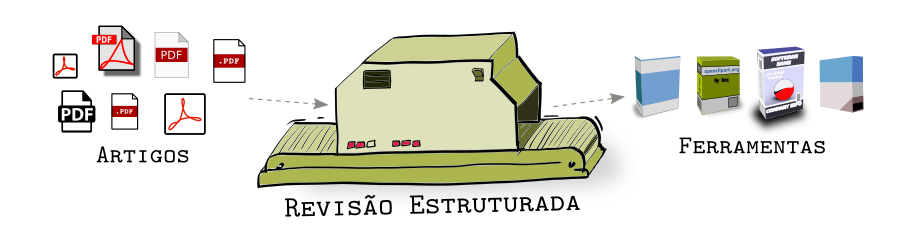
\includegraphics[scale=0.33]{imagens/revisao-estruturada.png}
  \caption{Representação gráfica da revisão estruturada}
  \label{figura-revisao-estruturada}
\end{figure}

Na primeira atividade da revisão estruturada são definidas as fontes de busca,
estas fontes são conferências que abordam o tema de interesse do estudo, e que
apresentam um grande potencial de encontrar ferramentas de software
do domínio de aplicação desejado. Esta primeira atividade de busca deve
incluir o maior número possível de ediçoes das conferências selecionadas, para
cada edição são copiados localmente todos os artigos em PDF para posterior
filtro na atividade seguinte.

A segunda atividade da revisão estruturada realizada em cima de todo o conjunto
de artigos é um filtro automática que busca em todo o conteúdo dos artigos os
termos de interesse, estes termos devem ser pensados em relaçao ao domínio de aplicação
desejado, devem ser abrangentes a fim de evitar falsos negativos.

A terceira e última atividade da revisão estruturada é a seleção de artigos,
nela será identificado se cada artigo resulta, de fato, em publicação de
ferramenta do domínio de aplicação. Esta seleção é feita a partir de uma
leitura superficial do artigo em busca de indícios de que o artigo publica uma
ferramenta e que o código-fonte desta ferramenta está disponível.

Uma vez identificados os artigos que publicaram ferramentas do domínio
desejado, procuramos no próprio artigo por referências de onde encontrar o
código-fonte da ferramenta. Neste momento, pode-se enfrentar algumas situações.

\begin{itemize}

  \item Os autores afirmam que a ferramenta está disponível mas o artigo
    não contém referências de onde encontrar o código-fonte, estes
    autores serão contactados, por email, solicitando informações de onde
    obter o código-fonte da ferramenta.

  \item O artigo indica onde obter o código-fonte da ferramenta, mas o acesso ao local
    indicado não está disponível, ou está disponível mas o software não se
    encontra lá, os autores serão contactados, solicitando informações
    atualizadas de onde obter uma cópia do código-fonte da ferramenta.

  \item Artigos que indicam onde obter o código-fonte da ferramenta e a referência
    está correta. Será feito o download do código-fonte da última versão
    disponível.

\end{itemize}

Uma vez que os autores contactados por email respondam com informações sobre
local onde obter o software, a ferramenta é adicionada ao conjunto de
ferramentas a serem analisadas. O código-fonte da versão mais recente de cada
uma destas ferramentas será copiado localmente para caracterização e análise
através da coleta de suas métricas de código-fonte.

\subsection{Ferramentas da indústria}

Em paralelo à revisão estruturada para seleção de ferramentas da academia será
realizada uma seleção manual não estruturada para busca de ferramentas da
indústria. O objetivo é aumentar o conjunto de objetos de estudo bem como ter
ferramentas de outros contextos além da academia, isto irá proporcionar uma
nova dimensão na caracterzação das ferramentas e permitirá realizar comparação
entre ferramentas de contextos distintos.

\subsection{Caracterização das ferramentas de análise estática}

As ferramentas de análise estática selecionadas serão caracterizadas
a partir de algumas dimensões que se mostrem necessárias ao nosso estudo, todas
as ferramentas foram obtidas em sua versão mais recente, apenas uma única versão
de cada ferramenta foi selecionada e será caracterizada a partir de tal versão,
esta cópia de cada ferramenta foi do seu código-fonte, algumas características
são obtidas do código-fonte, outras da documentação da ferramenta.

Esta caracterização será fundamental para compreender as métricas de código-fonte
extraídas destas ferramentas,
ferramentas que tenham interface gráfica de usuário por exemplo podem apresentar
valores diferentes daquelas que tenham apenas interface modo texto, suporte
a analisar múltiplas linguagens pode também trazer valores de métricas maiores ou
piores. Iremos levar estas características em consideração durante a análise
exploratória dos nosso dados.

Para compor as características e também evitar re-criar dimensões para características
de ferramentas deste domínio iremos nos basear no trabalho de
\citeonline{Novak2010}, onde um estudo para construção de uma taxonomia para
ferramentas de análise estática propuseram uma classificação a partir de uma
série de categorias.

Iremos utilizar algumas de suas características, apenas aquelas que nos forem necessárias
para interpretar e caracterizar a complexidade estrutural de tais ferramentas, segue abaixo todas
as características proposta no trabalho de \citeonline{Novak2010}.

\begin{description}

  \item {\it Entrada - quais tipos de arquivos podem ser carregados na ferramenta:}
    \begin{itemize}
      \item Código-fonte - arquivos de código texto podem ser carregados
      \item Byte code - arquivos com Java Byte Code ou Microsoft
      \item Linguagem intermediária (MSIL) pode ser carregada
    \end{itemize}

  \item {\it Lançamentos ({\it Releases}) - quantos lançamentos por ano:}
    \begin{itemize}
      \item Frequentemente $>=$ 3 vezes ao ano - novas versões da ferramenta são lançadas 3 ou mais vezes por ano
      \item Ocasionalmente $<$ 3 vezes ao ano - novas versões da ferramenta são lançadas menos que 3 vezes ao ano
      \item Obsoleta 0 vezes ao ano - intervalo entre novos lançamentos é maior que 1 ano
    \end{itemize}

  \item {\it Linguagens suportadas - quais linguagens de programação a ferramenta suporta:}
    \begin{itemize}
      \item .NET - todas as linguagens compiladas em bibliotecas ou programas no framework .NET
      \item VB .NET - suporta VB.NET
      \item C\# - suporta C\#
      \item Java - suporta linguagem de programação Java
      \item C, C++ - suporta linguagem de programação C ou C++
    \end{itemize}

  \item {\it Tecnologia - quais tecnologias são usadas para procurar erros no código:}
    \begin{itemize}
      \item Dataflow - busca por erros com dataflow
      \item Sintaxe - busca por errors de sintaxe e correctness
      \item Prova de teoremas - procurar erros em provar diferentes teoremas
      \item Verificação de modelos - procurar erros com verificação de modelo
    \end{itemize}

  \item {\it Regras - conjunto de regras, quais são suportadas por diferentes código estático:}
    \begin{itemize}
      \item Estilo - inspeciona a aparência do código-fonte
      \item Naming - checa se as varáveis são nomeadas corretamente (ortografia, padroes de nomenclatura, ...)
      \item Geral - regras gerais de analise estática de código
      \item Concorrencia - erros com execução de código de concorrente
      \item Exceções - erros lançando ou não exceções
      \item Performance - erros de performance das aplicações
      \item Interoperabilidade - erros de comportamento comum
      \item Segurança - erros que podem impactar na segurança da aplicação
      \item SQL - procurar por "SQL injections" e outros erros de SQL
      \item Buffer overflow - erros de segurança, que explorar buffer overflow
      \item Manutenabilidade - regras para melhor manutenabilidade da aplicação
    \end{itemize}

  \item {\it Configurabilidade - habilidade de configurar a ferramenta:}
    \begin{itemize}
      \item Documento texto - comfiguração é feita via documento texto
      \item XML - configuração pe feita por documento XML
      \item GUI - configuraçãi é feita via interface gráfica
      \item Ruleset - ferramenta pode ligar/desligar conjunto de regras
    \end{itemize}

  \item {\it Extensibilidade - se a ferramenta pode ser extendida com regras próprias:}
    \begin{itemize}
      \item Possível - é possível extender
      \item Não possível - não é possível extender
    \end{itemize}

  \item {\it Disponibilidade - de que forma a ferramenta está disponível:}
    \begin{itemize}
      \item Código Aberto ({\it Open Source}) - a ferrament é livre e o código-fonte está disponível
      \item Grátis ({\it Free}) - a ferramenta é grátis mas o código-fonte não está disponível
      \item Comercial - a ferramenta está disponível mediante pagamento
    \end{itemize}

  \item {\it Experiência do usuário - de que forma a ferramenta pode ser usada, como é oferecida:}
    \begin{itemize}
      \item Integração com ambiente - como a ferramenta é integrada ao ambiente de trabalho
      \item Localização automática de erros no código - quando a ferramenta encontra um erro, ela leva ao local do erro
      \item Ajuda abrangente sobre falhas - se a ferramenta oferece ajuda na resolução de erros
      \item Interface de usuário - disponibilidade de uma interface de usuário
      \item Linha de comando - ela pode ser executada via linha de comando
      \item GUI - a ferramente pode ser executada em uma interface gráfica (GUI)
    \end{itemize}

  \item {\it Saída - representação dos resultados da ferramenta:}
    \begin{itemize}
      \item Arquivo texto - ferramenta pode apresentar resultados em arquivos texto
      \item Lista - ferramenta pode apresentar resultados numa interface de usuário customizada controlada em GUI
      \item Arquivo XML - ferramenta pode apresentar resultados em dados XML
      \item Arquivo HTML - ferramenta pode apresentar resultados em dados HTML
    \end{itemize}

\end{description}

Iremos utilizar algumas destas categorias na caracterização das ferramentas
selecionadas neste estudo, e vamos também caracterizar em relação à algumas dimensões que nos
foram necessárias mas que não faziam parte das dimensões propostas por \citeonline{Novak2010},
estas dimensões são as seguintes.

\begin{description}

  \item {\it Linguagem de programação - em que linguagem de programação à ferramenta é escrita:}
    \begin{itemize}
      \item .NET
      \item VB .NET
      \item C\#
      \item Java
      \item C, C++
    \end{itemize}

  \item {\it Tamanho em número de classes - número de classes/módulos da ferramenta}

  \item {\it Contexto - onde a ferramenta surgiu:}
    \begin{itemize}
      \item Academia
      \item Indústria
    \end{itemize}

\end{description}

Além das características citadas iremos também caracterizar cada ferramente quando ao
seu nível de manutenabilidade através da interpretação das suas métricas de código-fonte.

Para cada uma das ferramentas selecionadas, iremos coletar suas métricas de código-fonte de
forma automatizada através da ferramenta Analizo, em seguida analisaremos seus valores em
comparação com as demais características.

\subsection{Analizo} \label{analizo}

Analizo é um conjunto de ferramentas para análise de código-fonte e
visualização, desenvolvido tendo como requisitos suportar múltiplas linguagens
de programação, ser software livre, ser extensível e que seja capaz de lidar
com código-fonte não mais compilável.

Este último requisito permite analisar código-fonte com erros de sintaxe, com
referências a bibliotecas não mais disponíveis, ou que usem bibliotecas com
mudanças de API em versões mais recentes. Isto é importante especialmente ao
analisar código-fonte legado em estudos sobre evolução de software.

Ela será a ferramenta utilizada por nós durante este estudo para análise do
código-fonte das ferramentas selecionadas, a decisão pela ferramenta Analizo
se deu por conta dela ser também a escolha utilizada nos trabalhos
relacionados (seção \ref{trabalhos-relacionados}) onde estamos nos apoiando,
além disso, Analizo também tem sido utilizada em diversos estudos
desenvolvidos em nosso grupo de pesquisa (seção \ref{trabalhos-analizo}).

\subsubsection{Arquitetura}

A arquitetura do Analizo é apresentada na Figura \ref{arquitetura-analizo}
através de uma representação do tipo {\it Layered Style} \cite{Clements2002},
onde cada camada no diagrama usa apenas os serviços oferecidos pela camada
diretamente abaixo dela.

\begin{figure}[h]
\center
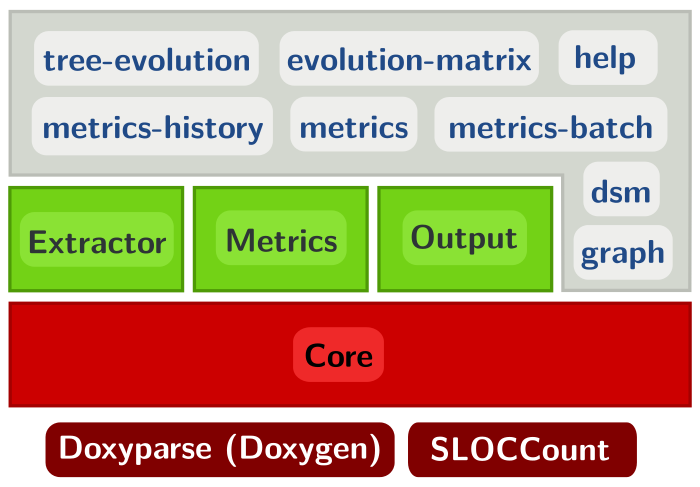
\includegraphics[scale=0.3]{imagens/analizo-architecture.png}
\caption{Arquitetura do Analizo, usando Layered Style \cite{Clements2002}}
\label{arquitetura-analizo}
\end{figure}

O {\it Core} contém as estruturas de dados usadas para armazenar informações a
respeito do código-fonte sendo analisado, como a lista de módulos\footnote{o
conceito ``módulo'' é usado como um termo abrangente para designar diferentes
tipos de estruturas usados em desenvolvimento de software, como classes e
arquivos fonte C}, elementos dentro de cada módulo (atributos, variáveis,
métodos, funções), informações de dependência (chamada, herança, etc). Esta
camada implementa a maior parte da lógica de negócio do Analizo, e não depende
de nenhuma outra camada.

A camada {\it Extractor} lida com as informaçoes de código-fonte obtidas pelas
diferentes estratégias implementadas no Analizo. Os extratores obtém
informações do código-fonte e armazenam em estruturas de dados da camada {\it
Core}. Adicionar um novo extrator requer apenas a criação de uma nova subclasse
que faça interface com uma ferramenta externa ou que ela própria realize análise
de código-fonte. Atualmente existem dois extratores, ambos fazem interface
com ferramentas externas de análise estática de código-fonte:

\begin{itemize}

  \item {\it Analizo::Extractor::Doxyparse} é uma interface para o Doxyparse,
  um parser de código-fonte para C, C++ e Java desenvolvida por nosso grupo de
  pesquisa\cite{Costa2009}. Doxyparse é baseado no
  Doxygen\footnote{doxygen.org}, um sistema de documentação multi-linguagem.

  \item {\it Analizo::Extractor::Sloccount} é uma interface para o
  Sloccount\footnote{dwheeler.com/sloccount} desenvolvido por David A. Wheeler,
  uma ferramenta que calcula o número efetivo de linhas de código.

\end{itemize}

As outras camadas intermediárias são {\it Metrics} e {\it Output}. A camada
{\it Metrics} processa as estruturas de dados do {\it Core} para calcular
métricas, até o momento Analizo suporta um conjunto razoável de métricas
(listadas na Seção \ref{metricas}), uma representação desta camada pode ser
vista no diagrama da Figura \ref{arquitetura-metrics-analizo}. A camada {\it
Output} é responsável por lidar com diferentes formatos de arquivos.
Atualmente, apenas o formato DOT é implementado no Analizo para representar
grafo de dependencia, adicionar novos formatos é simplesmente adicionar novas
classes nesta camada.

\begin{figure}[H]
\center
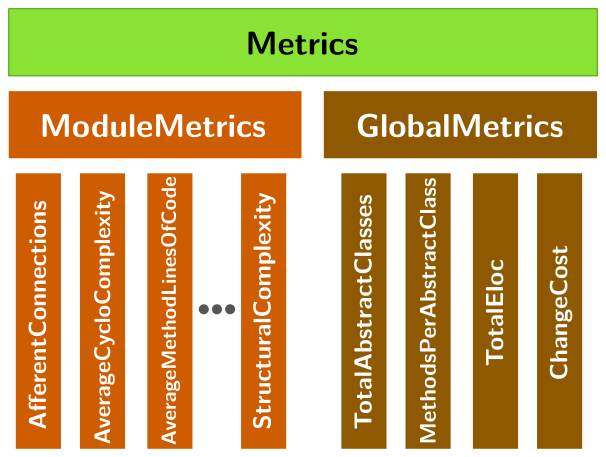
\includegraphics[scale=0.4]{imagens/analizo-metrics-architecture.png}
\caption{Arquitetura do módulo metrics em detalhe, usando Layered Style \cite{Clements2002}}
\label{arquitetura-metrics-analizo}
\end{figure}

A camada {\it Tools} fornece um conjunto de ferramentas de linha de comando que
constituem a interface do analizo, tanto para usuários finais quanto para
aplicações de mais alto nível. Estas ferramentas usam serviços providos pelas
outras camadas: eles instanciam as estruturas de dados do {\it Core},
inicializam um ou mais extratores, opcionalmente executam o processador de
métricas, instanciam um módulo de formato de saída, e gerencia todos eles para
prover o resultado desejado. A maioria das funcionalidades descritas na Seção
\ref{funcionalidades} são implementadas na camada {\it Tools} do Analizo.

Estas ferramentas são pensadas na filosofia UNIX: fazem uma tarefa
especializada e geram uma saída que pode ser utilizada como entrada para outras
ferramentas, seja para o próprio Analizo ou para ferramentas externas. Algumas das
ferramentas implementadas no Analizo são feitas consumindo saída gerada por
outra ferramenta ao invés de manipular explicitamente os internos do Analizo,
algumas outras são desenhadas para prover saída em formato específico para
aplicacoes externas, como por exemplo programas para desenho de grafos ou
visualização de dados.

\subsubsection{Funcionalidades}\label{funcionalidades}

{\bf Análise de código-fonte multi-linguagem}

Atualmente Analizo suporta análise de código-fonte escrito em C, C++ e Java.
Entretanto, pode ser facilmente estendido para suportar outras linguagens pois
pode potencialmente suportar as inúmeras outras linguagens suportadas pelo Doxygen.

{\bf Métricas}\label{metricas}

O Analizo suporta tanto métricas em nível de projeto, que é calculada para todo o projeto,
quanto métricas em nível de módulos, que é calculado individualmente para cada módulo.
No nível de projeto, Analizo também provê estatística descritiva básica para cada métrica em
nível de módulo: soma, média, mediana, moda, desvio padrão, variância, skewness e kurtosis da
distribuição, valores mínimo e maximo. As seguintes métricas são suportadas até o momento:

\begin{itemize}

  \item Métricas em nível de projeto: Change Cost, Total Abstract Classes,
  Total Coupling Factor, Total Effective Lines of Code, Total Lines of Code,
  Methods per Abstract Class, Total Number of Modules, Total number of modules
  with at least one defined attributes, Total number of modules with at least
  one defined method, Total Number of Methods.

  \item Métricas em nível de módulo: Afferent Connections per Class, Average
  Cyclomatic Complexity per Method, Average Method Lines of Code, Argument with
  'nonnull' attribute passed null, Average Number of Parameters per Method,
  Allocator sizeof operand mismatch, Assigned value is garbage or undefined,
  Bad deallocator, Bad free, Coupling Between Objects, Dead assignment,
  Divisions by zero, Double free, Depth of Inheritance Tree, Dereference of
  null pointer, Dereference of undefined pointer value, Potential buffer
  overflow in call to 'gets', Lack of Cohesion of Methods, Lines of Code,
  Memory leak, Max Method LOC, Number of Attributes, Number of Children, Number
  of Methods, Number of Public Attributes, Number of Public Methods,
  Out-of-bound array access, Offset free, Potential insecure temporary file in
  call 'mktemp', Response for a Class, Result of operation is garbage or
  undefined, Return of stack variable address, Stack address stored into global
  variable, Structural Complexity, Undefined allocation of 0 bytes,
  Use-after-free, Uninitialized argument value.

\end{itemize}

É possível especificar que certos diretórios dentro do projeto não devem ser
analisados, de forma que o Analizo ignore tais arquivos durante a análise e o
cálculo de métricas.

{\bf Processamento em lote}\label{lote}

A maioria dos estudos quantitativos em Engenharia de Software envolve aquisição
de métricas de código-fonte de um grande número de projetos, processar cada
projeto individualmente é pouco prático, passível de erros e difícil de
repetir. Analizo pode processar multiplos projetos em lote e produzir arquivo
de dados CSV com métricas de cada projeto, bem como um resumo com as métricas
em nível de projeto de todos os projetos. Estes arquivos de dados podem ser
facilmente importados em ferramentas de estatística ou planilhas para análise
futura. Esta capacidade de processar em lote pode também ser utilizada para
analisar várias versões de um mesmo projeto, especialmente útil em estudos
sobre evolução de software.

Este processamento em lote pode se beneficiar de processamento paralelo dando
mais agilidade e na análise e reduzindo o tempo total de processamento.  A
saída pode ser também escrita diretamente em um banco de dados relacional ao
invés de gerar arquivos CSV. Outro recurso voltado à performance é um sistema
de cache para as informações previamente calculadas, evitando repetição de
processamento.

{\bf Histórico de métricas}

Algumas vezes pesquisadores precisam processar o histórico de projetos de
software de uma forma mais escalável. Analizo pode processar repositórios de
controle de versão e prover arquivo de dados CSV com valores de métricas para
cada revisão onde o código-fonte foi alterado no projeto, ou pode também gravar
os valores diretamente num banco de dados ao invés de usar arquivos CSV. Repositórios Git e
Subversion são suportados diretamente, repositórios CVS devem ser convertidos
para Git de forma manual.

{\bf Grafo de dependência}

Analizo pode gerar saída com informações sobre dependência entre as entidades
do projeto em um formato adequado para processamento por ferramentas de
renderização de grafos do Graphviz\footnote{graphviz.org}. A Figura
\ref{sample-graph} apresenta um exemplo de grafo desenhado pela ferramenta {\it
dot} do Graphviz a partir da saída gerada pelo Analizo {\it graph}.

\begin{figure}[h]
\center
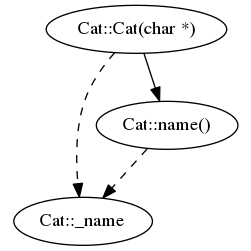
\includegraphics[scale=0.4]{imagens/sample-graph.png}
\caption{Exemplo de grafo de dependência}
\label{sample-graph}
\end{figure}

{\bf Matriz de evolução}

Outra funcionalidade útil do Analizo é a visualização de matrizes de evolução
\cite{Lanza2001}. Ao processar cada release de um projeto (ver Seção
\ref{lote}), o usuário pode solicitar a criação de uma matrix de evolução a
partir de arquivos de dados individuais. A Figura \ref{sample-evolution-matrix}
apresenta um exemplo de uma matrix produzida pelo Analizo.

\begin{figure}[h]
\center
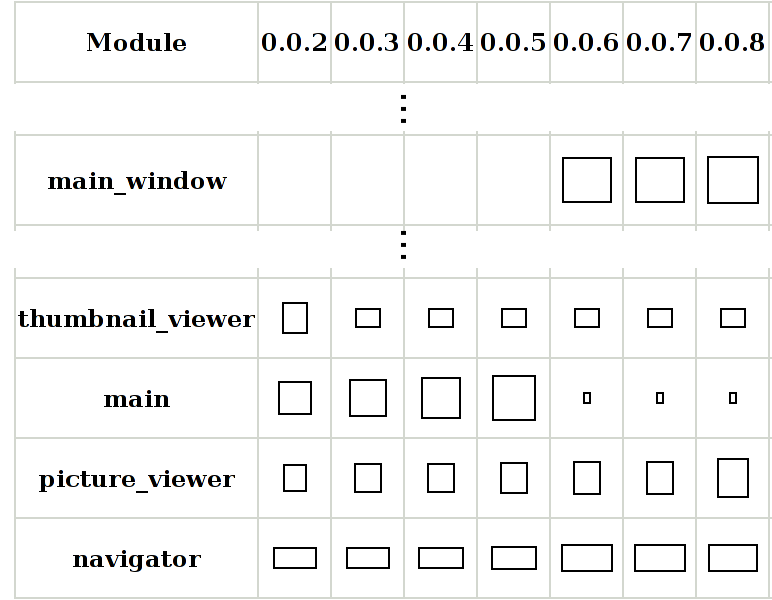
\includegraphics[scale=0.2]{imagens/sample-evolution-matrix.png}
\caption{Exemplo de matrix de evolução}
\label{sample-evolution-matrix}
\end{figure}

{\bf Matriz de estrutura de projeto}

Uma funcionalidade recente do Analizo é a representação visual do
relacionamento entre os módulos do projeto em forma de uma Matriz de estrutura
de projeto ({\it Design Structure Matrix}) \cite{Maccormack2006}, uma DSM é a
representação de um grafo de dependência em forma de uma matriz quadrada. Um
exemplo gerado pelo Analizo pode ser visto na Figura \ref{sample-dsm}.

\begin{figure}[h]
\center
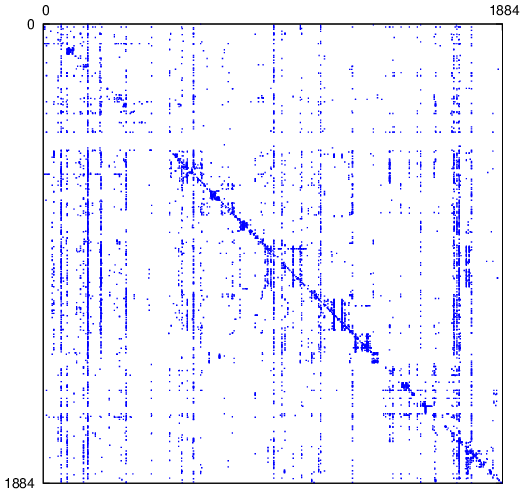
\includegraphics[scale=0.3]{imagens/sample-dsm.png}
\caption{Exemplo de matrix de estrutura de projeto}
\label{sample-dsm}
\end{figure}

\subsubsection{Uso em trabalhos de pesquisa}
\label{trabalhos-analizo}

Analizo tem sido extensivamente usada por nosso grupo de pesquisa em diversos
estudos:

\begin{itemize}

  \item \cite{Amaral2009} usou o grafo de dependencia gerado pelo Analizo para
  gerar uma matriz de evolução em um estudo de caso com o projeto VLC.

  \item \cite{Costa2009} fez uma comparação entre diferentes estratégias para
  extração de informação de dependencias entre módulos do código-fonte,
  resultando no desenvolvimento do Doxyparse - o extrator baseado no Doxygen do
  Analizo.

  \item \cite{Terceiro2009} usou métricas em um estudo exploratório sobre a
  evolução da complexidade estrutural em projetos de software livre escritos em
  C.

  \item \cite{Morais2009} usou a ferramenta de métricas do Analizo como backend
  para o Kalibro, um software para avaliação e observação de métricas de código-fonte.
  
  \item \cite{Terceiro2010} usou o processamento de histórico de métricas para
  realizar um estudo exploratório sobre a evolução da complexidade estrutural em
  7 projetos de servidor web de diferentes tamanhos.

  \item \cite{Meirelles2010} usou o processamento em lote do Analizo para
  processas o código-fonte de mais de 6000 projetos de software livre do
  repositório Sourceforge.net.

  \item \cite{Meirelles2011} usou o Analizo em um estudo sobre impacto de
  métricas de código-fonte na atratividade de projetos de softwares livres.

  \item \cite{Terceiro2012Understanding} usou o Analizo para investigar fatores
  que influenciam na evolução da complexidade estrutural em projetos de software
  livres.

  \item \cite{Silva2012} usou o Analizo para minerar 16000 revisões de
  repositórios de projetos de software para investigar o potencial de uma nova
  métrica chamada Lack of Concern-based Cohesion.

  \item \cite{Ronaldo2015} utilizou o Analizo para extrair métricas de
  código-fonte de 14 versões do sistema Android e estudar a evoluçao da API e
  seus aplicativos.

\end{itemize}

A maioria destes trabalhos contribuíram com melhorias para o Analizo, fazendo
dele ainda mais apropriado para pesquisas envolvendo análise de código-fonte.

\subsubsection{Considerações finais}

Analizo é útil tanto para pesquisadores trabalhando com análise de código-fonte
quanto para profissionais que precisam analisar seus projetos em busca de
potenciais problemas ou melhorias. Neste trabalho de mestrado utilizamos o
Analizo para coletar métricas de código-fonte das ferramentas de análise
estática selecionadas.

Analizo é software livre, licenciado sob a GNU General Public License versão 3.
Seu código-fonte, bem como pacotes binários, manuais e tutoriais podem ser
obtidos em http://analizo.org. Todas as ferramentas são auto-documentadas e
podem ser consultadas como páginas de manual UNIX. Analizo é escrito em Perl.
Sua última versão 1.19.1 foi lançada (no escopo deste trabalho) em 01 de
Setembro de 2016 e será a versão utilizada neste estudo.

\subsection{Análise dos dados} \label{analise}

Os dados coletados pelo Analizo incluem métricas de código-fonte para cada módulo/classe de
cada ferramenta selecionada, tanto da indústria quanto da academia. As
métricas a serem analisadas e interpretadas são as métricas descritas na Seção
\ref{metricas-de-codigo}.

Todos os cálculos utilizados neste trabalho estão disponíveis em nosso
repositório\footnote{http://github.com/joenio/dissertacao-ufba-2016} no arquivo
{\em
dataset/analyze-all-projects}\footnote{http://github.com/joenio/dissertacao-ufba-2016/blob/master/dataset/analyze-all-projects}.

Com isto podemos analisar os dados das métricas para cada uma das ferramentas analisadas.
Estes valores serão compreendidos e validados através de uma interpretação manual.

Os valores encontrados serão avaliados sempre tendo em vista os intervalos
sugeridos na Tabela \ref{valores-frequentes}, esta tabela traz os valores encontrados
no estudo que estamos replicando em parte\cite{Meirelles2013}.

\begin{table}[H]
  \caption{Valores frequentes\cite{Meirelles2013}}
  \centering
  \begin{tabular}{| c | l | l | l | l | l |}
    \hline
    Métrica           & Linguagem & Muito frequente & Frequente & Pouco frequente & Não frequente \\
    \hline
\multirow{3}{*}{CBO}   & C         & 0 -- 5,0   & 6,0 -- 9,0   & 9,0 -- 12,0  & $>$ 12,0  \\
                       & C++       & 0 -- 3,0   & 4,0 -- 5,0   & 6,0 -- 7,0   & $>$ 7,0   \\
                       & Java      & 0 -- 3,0   & 4,0 -- 6,0   & 7,0 -- 9,0   & $>$ 9,0   \\
    \hline
\multirow{3}{*}{LCOM4} & C         & 0 -- 5,0   & 6,0 -- 12,0  & 12,0 -- 20,0 & $>$ 20,0  \\
                       & C++       & 0 -- 5,0   & 6,0 -- 10,0  & 10,0 -- 14,0 & $>$ 14,0  \\
                       & Java      & 0 -- 3,0   & 4,0 -- 7,0   & 8,0 -- 12,0  & $>$ 12,0  \\
    \hline
\multirow{3}{*}{SC}    & C         & 0 -- 18,0  & 19,0 -- 77,0 & 78,0 -- 168,0 & $>$ 168,0 \\
                       & C++       & 0 -- 12,0  & 13,0 -- 28,0 & 29,0 -- 51,0  & $>$ 51,0  \\
                       & Java      & 0 -- 6,0   & 7,0 -- 21,0  & 22,0 -- 45,0  & $>$ 45,0  \\
    \hline
  \end{tabular}
  \label{valores-frequentes}
\end{table}

\section{Analysis procedure}

\section{Evaluation of validity}
